\documentclass[a4,useAMS,usenatbib,usegraphicx]{mn2e} 
%\documentclass{latex/emulateapj} 
%External Packages and personalized macros
%=========================================================================
%		EXTERNAL PACKAGES
%=========================================================================
\usepackage{amsmath} 
\usepackage{amssymb} 
%\usepackage[section]{placeins}
\usepackage {graphicx}
%\usepackage{graphics}
\usepackage[dvips]{epsfig}
\usepackage{epsfig}  
\usepackage{color}
\usepackage[normalem]{ulem}
\usepackage{hyperref}
\usepackage{caption}
%Non reposionated tables
\usepackage{float}
\restylefloat{table}
%Multiple columns support for tables
\usepackage{array}
\usepackage{booktabs}
\setlength{\heavyrulewidth}{1.5pt}
\setlength{\abovetopsep}{4pt}
\pdfminorversion=5

%=========================================================================
%		INTERNAL MACROS
%=========================================================================
\def\be{\begin{equation}}
\def\ee{\end{equation}}
\def\ba{\begin{eqnarray}}
\def\ea{\end{eqnarray}}

% To highlight comments 
\definecolor{red}{rgb}{1,0.0,0.0}
\newcommand{\red}{\color{red}}
\definecolor{darkgreen}{rgb}{0.0,0.5,0.0}
\newcommand{\SRK}[1]{\textcolor{darkgreen}{\bf SRK: \textit{#1}}}
\newcommand{\SRKED}[1]{\textcolor{darkgreen}{\bf #1}}
\newcommand{\before}[1]{\textcolor{red}{ #1}}
\newcommand{\after}[1]{\textcolor{darkgreen}{ #1}}

\newcommand{\LCDM}{$\Lambda$CDM~}
\newcommand{\beq}{\begin{eqnarray}}  
\newcommand{\eeq}{\end{eqnarray}}  
\newcommand{\zz}{$z\sim 3$} 
\newcommand{\apj}{ApJ}  
\newcommand{\jcap}{JCAP}  
\newcommand{\apjs}{ApJS}  
\newcommand{\apjl}{ApJL}  
\newcommand{\aj}{AJ}  
\newcommand{\mnras}{MNRAS}  
\newcommand{\mnrassub}{MNRAS accepted}  
\newcommand{\aap}{A\&A}  
\newcommand{\aaps}{A\&AS}  
\newcommand{\araa}{ARA\&A}  
\newcommand{\nat}{Nature}  
\newcommand{\physrep}{PhR}
\newcommand{\pasp}{PASP}    
\newcommand{\pasj}{PASJ}    
\newcommand{\avg}[1]{\langle{#1}\rangle}  
\newcommand{\ly}{{\ifmmode{{\rm Ly}\alpha}\else{Ly$\alpha$}\fi}}
\newcommand{\hMpc}{{\ifmmode{h^{-1}{\rm Mpc}}\else{$h^{-1}$Mpc}\fi}}  
\newcommand{\hGpc}{{\ifmmode{h^{-1}{\rm Gpc}}\else{$h^{-1}$Gpc}\fi}}  
\newcommand{\hmpc}{{\ifmmode{h^{-1}{\rm Mpc}}\else{$h^{-1}$Mpc}\fi}}  
\newcommand{\hkpc}{{\ifmmode{h^{-1}{\rm kpc}}\else{$h^{-1}$kpc}\fi}}  
\newcommand{\hMsun}{{\ifmmode{h^{-1}{\rm {M_{\odot}}}}\else{$h^{-1}{\rm{M_{\odot}}}$}\fi}}  
\newcommand{\hmsun}{{\ifmmode{h^{-1}{\rm {M_{\odot}}}}\else{$h^{-1}{\rm{M_{\odot}}}$}\fi}}  
\newcommand{\Msun}{{\ifmmode{{\rm {M_{\odot}}}}\else{${\rm{M_{\odot}}}$}\fi}}  
\newcommand{\msun}{{\ifmmode{{\rm {M_{\odot}}}}\else{${\rm{M_{\odot}}}$}\fi}}  
\newcommand{\lya}{{Lyman$\alpha$~}}
\newcommand{\clara}{{\texttt{CLARA}}~}
\newcommand{\rand}{{\ifmmode{{\mathcal{R}}}\else{${\mathcal{R}}$ }\fi}}  
%SAMPLES
\newcommand{\GHBDM}{\texttt{GH}$_{\mbox{\tiny{BDM}}}$ }
\newcommand{\GHFOF}{\texttt{GH}$_{\mbox{\tiny{FOF}}}$ }
\newcommand{\IHBDM}{\texttt{IH}$_{\mbox{\tiny{BDM}}}$ }
\newcommand{\IHFOF}{\texttt{IH}$_{\mbox{\tiny{FOF}}}$ }
\newcommand{\PBDM}{\texttt{P}$_{\mbox{\tiny{BDM}}}$ }
\newcommand{\PFOF}{\texttt{P}$_{\mbox{\tiny{FOF}}}$ }
\newcommand{\IPBDM}{\texttt{IP}$_{\mbox{\tiny{BDM}}}$ }
\newcommand{\IPFOF}{\texttt{IP}$_{\mbox{\tiny{FOF}}}$ }
\newcommand{\RIPBDM}{\texttt{RIP}$_{\mbox{\tiny{BDM}}}$ }
\newcommand{\RIPFOF}{\texttt{RIP}$_{\mbox{\tiny{FOF}}}$ }


%MY COMMANDS #############################################################
\newcommand{\sub}[1]{\mbox{\scriptsize{#1}}}
\newcommand{\dtot}[2]{ \frac{ d #1 }{d #2} }
\newcommand{\dpar}[2]{ \frac{ \partial #1 }{\partial #2} }
\newcommand{\pr}[1]{ \left( #1 \right) }
\newcommand{\corc}[1]{ \left[ #1 \right] }
\newcommand{\lla}[1]{ \left\{ #1 \right\} }
\newcommand{\bds}[1]{\boldsymbol{ #1 }}
\newcommand{\oiint}{\displaystyle\bigcirc\!\!\!\!\!\!\!\!\int\!\!\!\!\!\int}
\newcommand{\mathsize}[2]{\mbox{\fontsize{#1}{#1}\selectfont $#2$}}
\newcommand{\eq}[2]{\begin{equation} \label{eq:#1} #2 \end{equation}}
\newcommand{\lth}{$\lambda_{th}$ }
\newcommand{\reff}{{\ifmmode{r_{\mbox{\tiny eff}}}\else{$r_{\mbox{\tiny eff}}$}\fi}}
%#########################################################################

\begin{document}

%=========================================================================
%		FRONT MATTER
%=========================================================================
\title[Halo concentration via the integrated mass profile]{Estimating dark matter  halo concentration using the integrated mass profile} 
\author[C.N. Poveda-Ruiz, J.E. Forero-Romero, J.C. Mu\~noz-Cuartas]{
\parbox[t]{\textwidth}{\raggedright 
  C. N. Poveda-Ruiz \thanks{cn.poveda542@uniandes.edu.co}$^{1}$
  J. E. Forero-Romero \thanks{je.forero@uniandes.edu.co}$^{1}$
  J. C. Mu\~noz-Cuartas \thanks{juan.munozc@udea.edu.co}$^{2}$
}
\vspace*{6pt}\\
$^1$Departamento de F\'{i}sica, Universidad de los Andes, Cra. 1
No. 18A-10, Edificio Ip, Bogot\'a, Colombia\\
$^2$Instituto de F\'{\i}sica - FCEN, Universidad de Antioquia, Calle
67 No. 53-108, Medell\'{\i}n, Colombia
}

\maketitle

\begin{abstract}
We present a new algorithm to estimate the concentration of N-body
dark matter halos using the integrated mass profile.
The method uses the full particle information without any binning,
making it reliable in cases when low numerical resolution becomes a
limitation for other methods.   
We test the performance of this method by estimating halo
concentration both on mock and N-body halos. 
We compare these results against two other methods:
maximum radial velocity measurements and radial particle binning.
Tests on the mock halos show that the accuracy of the new method to
recover known input concentrations varies with halo resolution,
outperforming the other two methods. 
We also measure the mass-concentration relationship on N-body
data. 
We find that in the probed mass range ($10^{12}\hMsun <
10^{14}\hMsun$) the three methods give consistent results within the
statistical uncertainties.   
We only find a small deviation at low masses, $M<10^{13}\hMsun$, where
the new method yields lower median concentration values by $20\%-30\%$
compared to the velocity and density methods. 
From these results we believe that the new method is a promising tool
to probe the internal structure of dark matter halos.
\end{abstract}

\begin{keywords}
Cosmology: theory, large-scale structure of Universe --
Methods: data analysis, numerical 
\end{keywords}


%*************************************************************************
\section{Introduction}
\label{sec:introduction}
%*************************************************************************
In the current structure formation paradigm the properties of galaxies
are coupled to the evolution of their dark matter (DM) hosting halo.
For instance, the sizes and dynamics of galaxies are determined by
the DM distribution inside a halo. This motivates the detailed study
a DM halo internal structure. 

The internal DM distribution in a halo can be parameterized through the density
profile.  
In a first approximation this profile is spherically symmetric and
its density only depends on the radial coordinate. 
One the most popular radial parameterizations is the
Navarro-Frenk-White (NFW) profile 
\citep{NFW}.   
If one is not interested in the very central region of the
dark matter halo (where galaxy formation takes place, and where the
effects of baryon physics on dark matter distribution are still 
unknown) one can also assume that this profile is universal.
\citep{Navarro2010}.  
 This profile is a double power law in radius, where the transition
break happens at the so-called scale radius, $r_s$.  
The ratio between the scale radius and the halo virial radius $R_v$ is
known as the concentration $c=R_v/r_s$. 


The concentration of the NFW profile provides the conceptual
framework to study simulated dark matter halos as a function of
redshift and cosmological parameters.
In many numerical studies 
\citep{Neto2007,Maccio2008,Duffy2008,Munoz2011,Prada2012,Ludlow2014} 
the results are summarized through the
mass-concentration relationship; that is the distribution of
concentration values at a fixed halo mass and redshift.
The success of such numerical experiments rests on a
reliable algorithm to estimate the concentration. 
Such an algorithm should provide unbiased results and must be robust
when applied to simulations of different numerical resolution.  

There are two main algorithms to estimate the concentration parameter
of a N-body dark matter halo. 
The first method takes the halo particles and bins them into
logarithmic radii to estimate the density in each bin, then it 
proceeds to fit the density as a function of the radius to the NFW
profile.  
A second method uses an analytic property of the NFW profile
that relates the maximum of the ratio of the circular velocity to the
virial velocity, $V_{\rm circ}$/$V_{\rm vir}$.  The concentration can
be then found as the root of an algebraic equation dependent on this
maximum value.  

The first method is straightforward to apply but presents two
disadvantages.  
First, it requires a large number of particles in
order to have a proper density estimate in each bin.  
This makes the method robust only for halos with at least $10^3$ particles.  
The second problem is that there is not a way to estimate the optimal
radial bin size, different choices may produce different results for the
concentration.

The second method solves the two problems mentioned above.  
It works with low particle numbers and does not involve data binning.  
However, it effectively takes into account only a single data point and
discards the behavior of the ratio $V_{\rm circ}/V_{\rm vir}$ below
and above its maxima.  
Small fluctuations on the value of this maximum can yield large
perturbations on the estimated concentration parameter.  

In this letter we present a third alternative based on fitting the
integrated mass profile.
This approach has two advantages with respect to the above mentioned
methods.  
It does not involve any data binning and does not throw away data
points. 
This translates into a robust estimate even at low resolution/particle
numbers.   
Furthermore, since the method does not require any binning, there is
no need to tune numerical parameters.
This provides a new independent method to estimate the concentration
parameter.   
Here we provide a detailed description of the method and a
comparison against the two traditional techniques by measuring its
performance both on mock and N-body halos.





\section{Basic properties of the NFW density profile}
\label{sec:basics}

Let us review first the basic properties of the NFW density profile.
This shall help us to define our notation.


\subsection{Density profile}

The NFW density profile can be written as

\begin{equation}
\rho(r) = \frac{\rho_c\delta_c}{r/r_s(1+r/r_s)^2},
\label{eq:definition}
\end{equation}
%
where $\rho_c\equiv 3H^2/8\pi G$ is the Universe critical density, $H$
is the Hubble constant, $G$ and the universal gravitational constant,
$\delta_c$ is the halo dimensionless characteristic density and $r_s$
is the scale radius. 
This radius marks the point where the logarithmic slope of the density
profile is equal to -2, the transition between the power law
scaling $\rho\propto r^{-1}$ for $r<r_s$ and $\rho\propto r^{-3}$ for
$r>r_s$. 

We define the virial radius of a halo, $r_v$, as the boundary of the
spherical volume that encloses a density of $\Delta_h$ times the mean
density of the Universe.  
The corresponding mass $M_{v}$, the virial mass, can be written as
$M_{v} = \frac{4\pi}{3}\bar{\rho}\Delta_h r_v^3$.  
From these virial quantities we define new dimensionless variables for
the radius and mass $x\equiv r/r_v$ and $m\equiv M(<r)/M_v$. 

In this letter we use $\Delta_h=740$, a number roughly corresponding to
200 times the critical density at redshift z=0.


\subsection{Integrated mass profile}

From these definitions we can compute the total mass enclosed inside a
radius $r$:
\begin{equation}
M(<r) = 4\pi\rho_c\delta_c  r_s^3\left[\ln \left
  (\frac{r_s+r}{r_s}\right) - \frac{r}{r_s+r}\right],
\end{equation}
%
or in terms of the dimensionless mass and radius variables

\begin{equation}
m(<x) =
\frac{1}{A}\left[\ln\left(1+xc\right)-\left(\frac{xc}{xc+1}\right)\right],
\label{eq:profile}
\end{equation}
%
where
%
\begin{equation}
A=\ln\left(1+c\right)-\left(\frac{c}{c+1}\right),
\end{equation}
%
and the parameter $c$ corresponds to the concentration $c\equiv r_v/r_s$.

From this normalization and for later convenience we define the
following function
%
\begin{equation}
f(x) = \ln\left(1+x\right)-\left(\frac{x}{x+1}\right).
\label{eq:f_NFW}
\end{equation}
%
The most interesting feature of Eq. (\ref{eq:profile}) is that the
concentration is the only free parameter to describe the integrated
mass profile.
 
\subsection{Circular velocity profile}

It is also customary to express the mass of the halo in terms of the
circular velocity $V_{c}=\sqrt{GM(<r)/r}$.
From this we can define a new dimensionless circular velocity $v(<x)\equiv
V_{c}(<r)/V_{c}(<r_v)$, using the result in Eq. \ref{eq:profile}
we have:

\begin{equation}
v(<x)=\sqrt{\frac{1}{A}\left[\frac{\ln\left(1+xc\right)}{x}-\frac{c}{xc+1}\right]},
\end{equation}
%
This normalized profile always shows a maximum provided that the
concentration is larger than $c>2$.
It is possible to show that for the NFW profile the maximum is
provided by

\begin{equation}
\mathrm{max}(v(<x)) = \sqrt{\frac{c}{x_{\rm max}}\frac{f(x_{\rm
      max})}{f(c)}},
\label{eq:max_v}
\end{equation}
where $x_{\rm max}=2.163$ \citep{Klypin2014} and the function $f(x)$
corresponds to the definition in Eq. (\ref{eq:f_NFW}).

\section{Methods to estimate the concentration from N-body simulations}
\label{sec:method}

\subsection{Estimates from the density and velocity profiles}

To date, there are two standard methods to estimate concentrations in
dark matter halos extracted from N-body simulations. 

The first method tries to directly estimate the density profile.  
It takes all the particles in the halo and bins them in the logarithm of
the radial coordinate from the halo center.  
Then, it estimates the density in each logarithmic bin counting the
particles and dividing by the corresponding shell volume.  
At this point is possible to make a direct fit to the density as a
function of the radial coordinate. 
This method has been broadly used for more than two decades to study
the mass-concentration-redshift relation of dark matter halos.
 
A second method uses the circular velocity profile.  
It finds the value of $x$ for which the normalized circular velocity
$v(<x)$ shows a maximum.  
Using this value it solves numerically for the corresponding value of
the concentration using Eq. (\ref{eq:max_v}). 
This method has been most recently used by \cite{Klypin2014} to study
the mass-concentration-redshift relation using the Multidark
Simulation Suite. 


\subsection{Our proposal: estimate from the integrated mass profile}

The new method uses the integrated mass profile defined in
Eq. (\ref{eq:profile}).
We build it from N-body data following the next steps.
First, we define the center of the halo to be at the position of the
particle with the lowest gravitational potential.  
Then we rank the particles by their increasing radial distance from
the center. 
From this ranked list of $i=1,N$ particles, the total mass at a radius
$r_i$ is $M_i=i\times m_p$, where $r_i$ is the position of the $i$-th
particle and $m_p$ is the mass of a single computational particle. 
In this process we discard the particle at the center. 

We divide the enclosed mass mass $M_i$ and the radii $r_i$ by their
virial values to obtain the dimensionless variables $m_i$ and $x_i$.
Once the mass profile is expressed in dimensionless variables the
concentration is the only free parameter. 
We then use an Affine Invariant Markov Chain Monte Carlo implemented in the
python module {\em emcee} \citep{emcee} to sample the likelihood
function distribution defined by ${\cal L}(c)\propto
\exp(-\chi^2(c)/2)$ where the $\chi^2(c)$ is 
written as

\begin{equation}
\chi^2(c)= \sum_{i=1}^{N}[\log m_i - \log m(< x_i;c)]^2,
\end{equation}
%
where $m(<x_i;c)$ corresponds to the values in Eq.(\ref{eq:profile})
at $x=x_i$ for a given value of the concentration parameter $c$ and
the $i$ index sums over all the particles in the numerical profile.
From the $\chi^2$ distribution we find the optimal value of the
concentration and its associated uncertainty.


\section{Results}
\label{sec:results}

We apply the three methods mentioned above on two different halo
samples.
The first sample is composed by mock halos generated to have known
concentration values in perfect spherical symmetry following an NFW
profile.    
Using this sample we want to quantify the ability to recover the
expected concentration as a function of particle number.
The second sample comes from a publicly available N-body cosmological
simulation.  
In this way we test the new method on more realistic and complex
data. 
We summarize the results on this dataset by showing the impact on the
mass-concentration relationship.



\subsection{Mock halo sample}

\begin{figure}
\begin{center}
  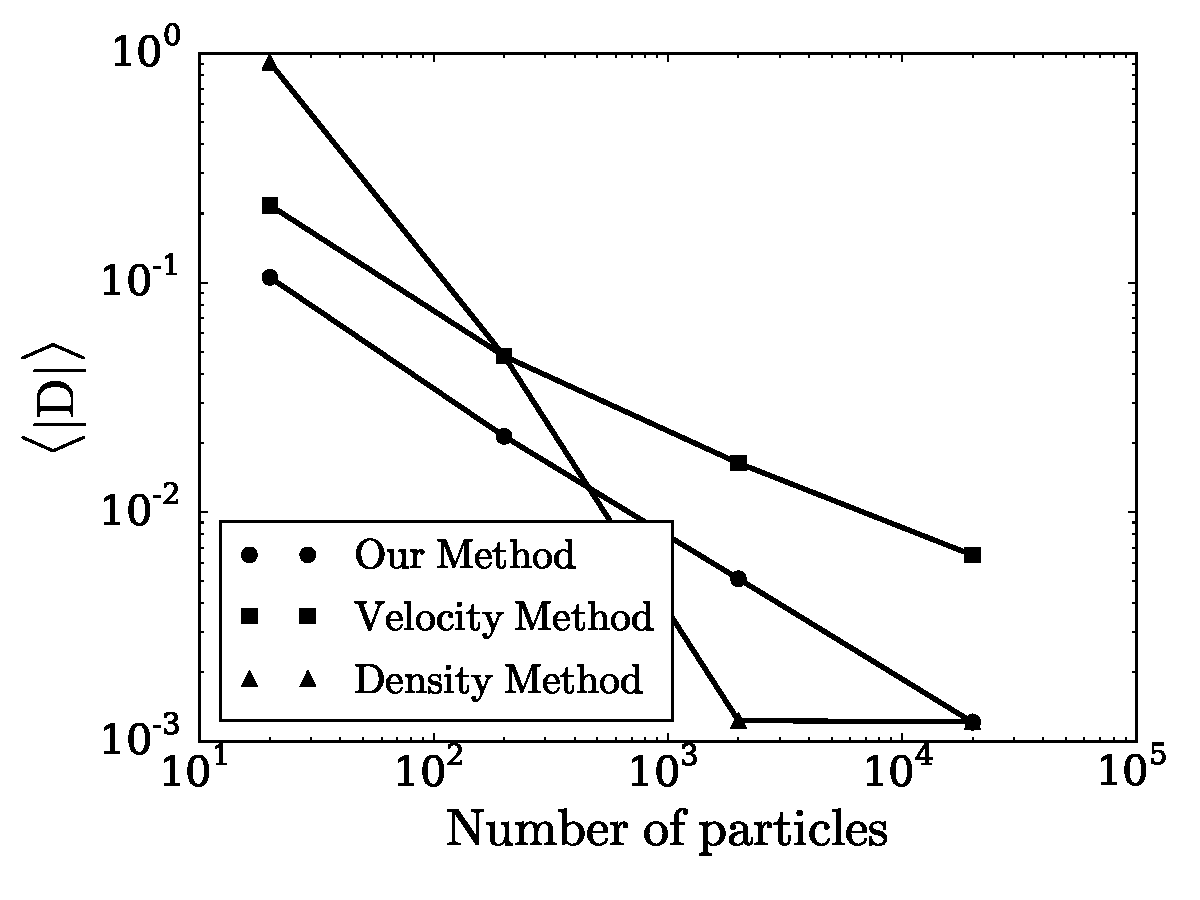
\includegraphics[width=0.50\textwidth]{error.pdf}
\end{center}
\vspace{-0.5cm}
\caption{Average value of the relative error in the concentration
  estimate, $\avg{|D|}$, as a function of the particle number $N$ in
  the set of mock halos. Different symbols represent different
  methods. The new method provides the most accurate estimate at fixed
  particle number.  
    \label{fig:error}}
\end{figure}

\begin{figure*}
\begin{center}
  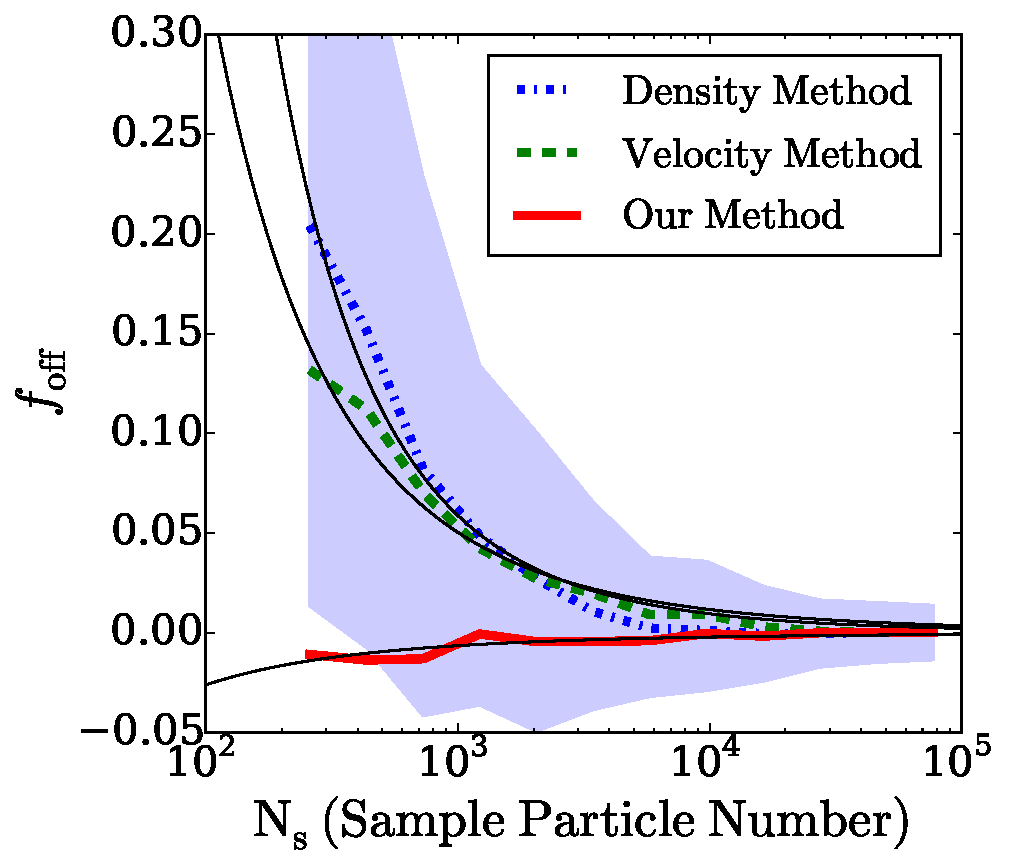
\includegraphics[width=0.47\textwidth]{avg_foff_bolshoi.pdf}
  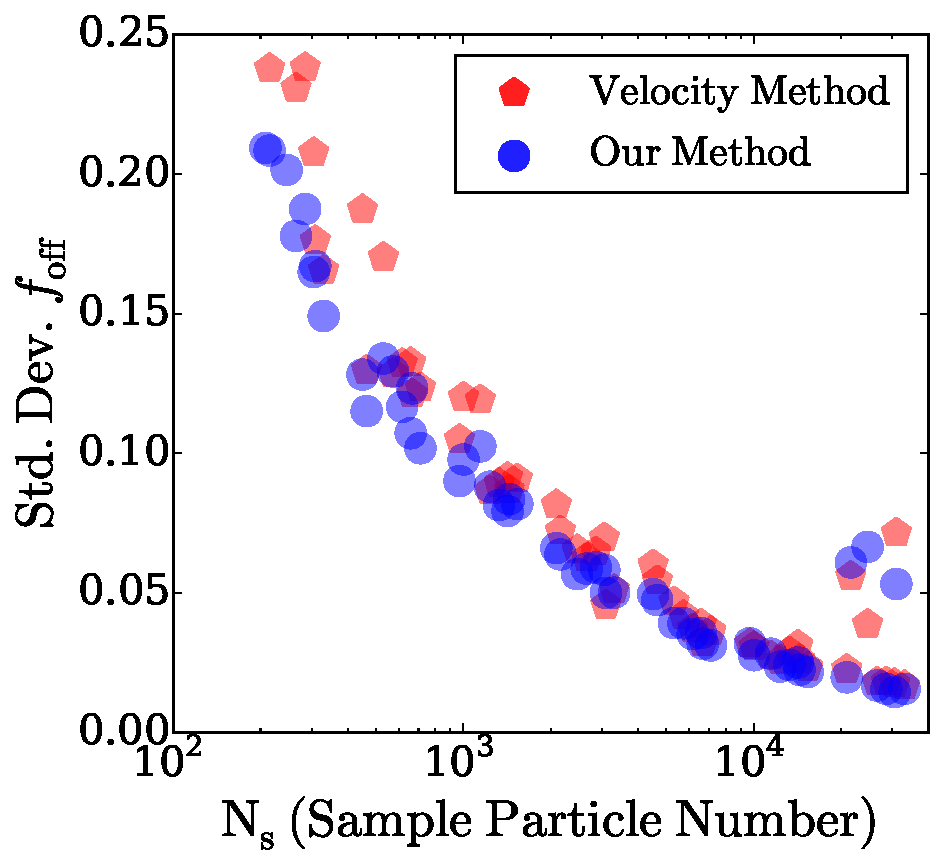
\includegraphics[width=0.45\textwidth]{stddev_foff_bolshoi.pdf}
\end{center}
\vspace{-0.5cm}
\caption{Average value of the relative error in the concentration
  estimate, $\avg{|D|}$, as a function of the particle number $N$ in
  the set of mock halos. Different symbols represent different
  methods. The new method provides the most accurate estimate at fixed
  particle number.  
    \label{fig:error}}
\end{figure*}



%\label{sec:data}
%\begin{figure*}
%  \begin{center}
%    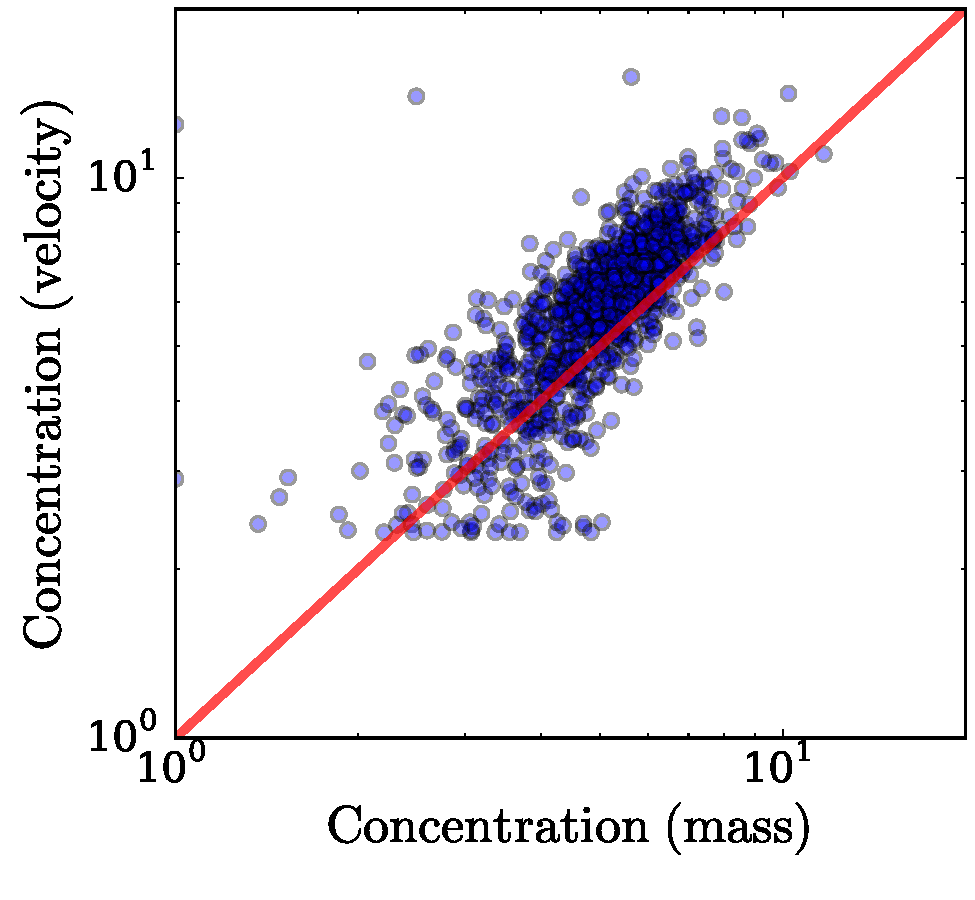
\includegraphics[width=0.32\textwidth]{conc_mass_vel.pdf}
%    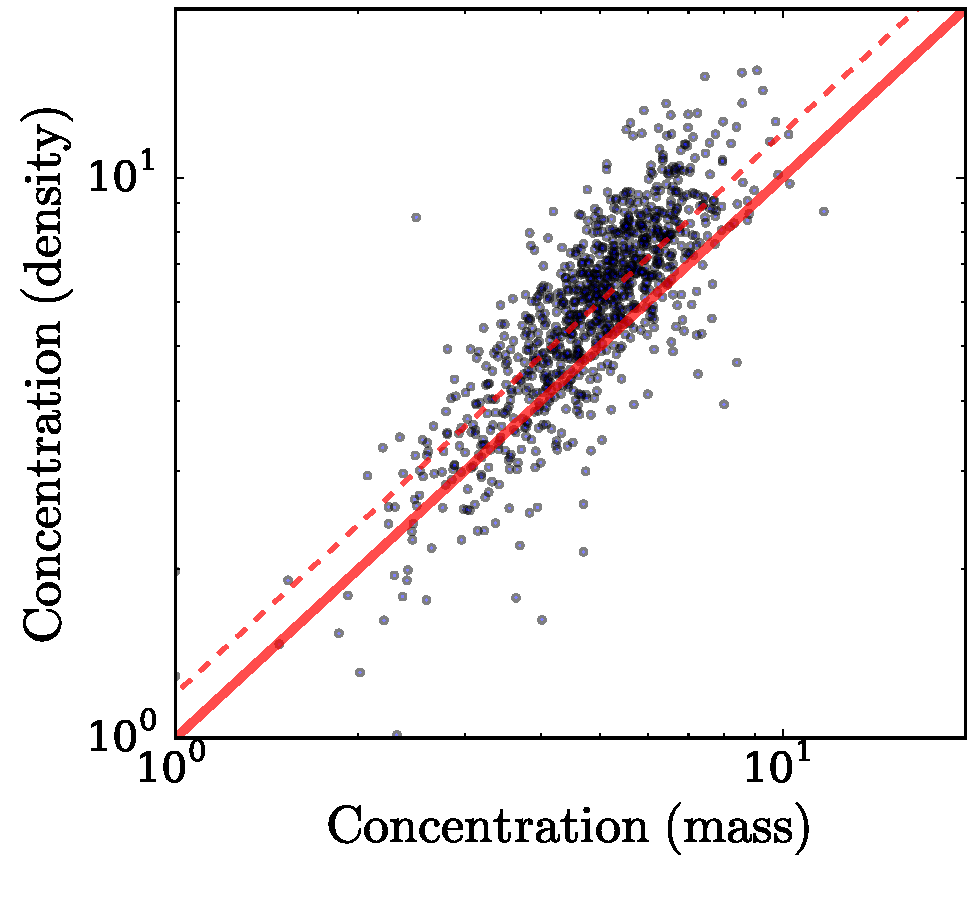
\includegraphics[width=0.32\textwidth]{conc_mass_dens.pdf}
%    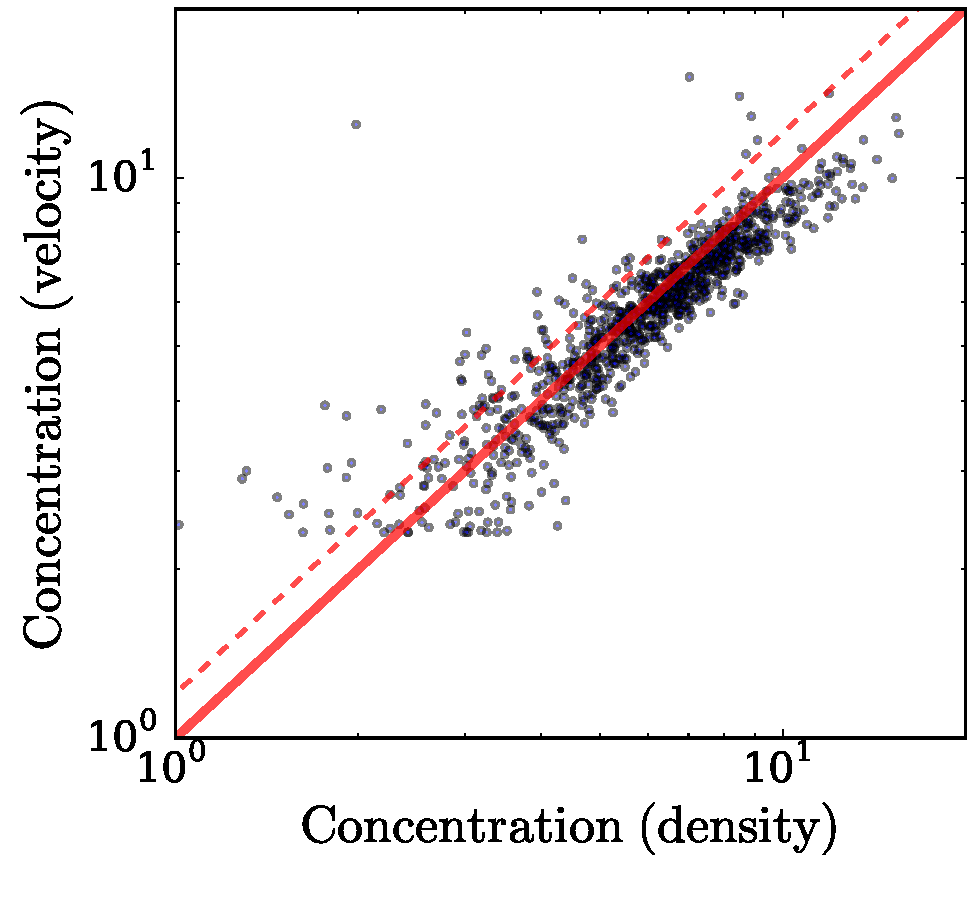
\includegraphics[width=0.32\textwidth]{conc_dens_vel.pdf}
%  \end{center}
%\vspace{-0.5cm}
%  \caption{Comparison between the concentrations measured by the new 
%    method and the maximum velocity (left) and density (middle)
%    methods. The solid line indicates the equal value between the two
%    techniques. The dashed line shows the upper 15 per cent difference
%    between two methods.
%  \label{fig:comparison}}
%\end{figure*}



The method we use to generate the mock halos is based on the
integrated mass profile.  
We start by fixing the desired concentration $c$ and total number of
particles $N$ in the mock halo.  
With these values we define the mass element as $\delta m = 1/M$, corresponding
to the mass of each particle such that the total mass is one.   
Then for each particle, $i=1,\ldots,N$, we find the value of $r_i$
such that the difference 
% 
\begin{equation}
m(<r_i;c) - i \cdot \delta m
\end{equation}
%
is zero using Ridders' method.

The value of $r_i$ is the radius of the $i$-th particle of the mock
halo.  
Then we generate random polar and azimuthal angles $\theta$ and
$\phi$ for each particle to ensure spherical symmetry.  
Finally these three spherical coordinates are transformed into
Cartesian coordinates $(r,\theta,\phi) \rightarrow (x,y,z)$.

We generate in total $400$ mock halos split into four different groups
of $100$ halos each.  
The four groups differ in the total number of particles for their
halos: $20$, $200$, $2000$ and $20000$.   
Inside each group the halos have random concentration values in the range
$1<c<20$ with a uniform distribution.  
We find the concentration values for all these halos using the
density, velocity and integrated mass methods described in the
previous section.    

We quantify the difference between the expected $c_{in}$ and measured
$c_{out}$ values by 
%
\begin{equation}
D=(c_{in}-c_{out})/c_{in},
\label{eq:D}
\end{equation}
%
and
%
\begin{equation}
\avg{|D|}=\frac{1}{\left|{\cal{H}}\right|}\sum_{{\cal{H}}} |D|,
\end{equation}
%
where ${\cal{H}}$ corresponds to a set of mock halos, and
$\left|{\cal{H}}\right|$ is the number of haloes in ${\cal{H}}$. 
A large discrepancy between the estimated and input concentrations are
quantified by a large $\avg{|D|}$.



Figure \ref{fig:error} shows the behaviour of $\avg{|D|}$ as a function of
halo particle number for the three different methods.

At fixed particle numbers the new method always shows the lowest
$\avg{|D|}$ values compared to the other two.
Its accuracy is on the order of $10\%$ for $20$ particles in the halo,
decreasing to $0.01\%$ for halos with $20000$ particles.  
The dependence of $\avg{|D|}$ with the particle number $N$
goes approximately as $\avg{|D|}\propto N^{-1/2}$.   
This hints that the increasing accuracy of the method could be due to
a decrease of Poisson noise. 

The method based on the maximum of the circular velocity shows a
similar behaviour with $\avg{|D|}\propto N^{-1/3}$.  
Its accuracy is $2-5$ times lower than in the new method, on the order of
$20\%$ for $20$ particle halos and $0.5\%$ for $20000$ particle
halos. 
The method  based on the direct density fit shows the lowest accuracy for a low
  particle number. 
  As it is discussed in \citep{Munoz2011}, density binning for halos
  with particle numbers below $\sim200$ leads to a biased estimation
  of the mass density profile, and therefore to a biased estimation of
  the concentration parameter. 
This behaviour is evident in the large values of $\avg{|D|}$ for halos
with number of particles below $\sim 200$ and an intermediate accuracy
between the other two methods for a high particle number. 

\subsection{Halos from a cosmological simulation}


\begin{figure*}
\begin{center}
  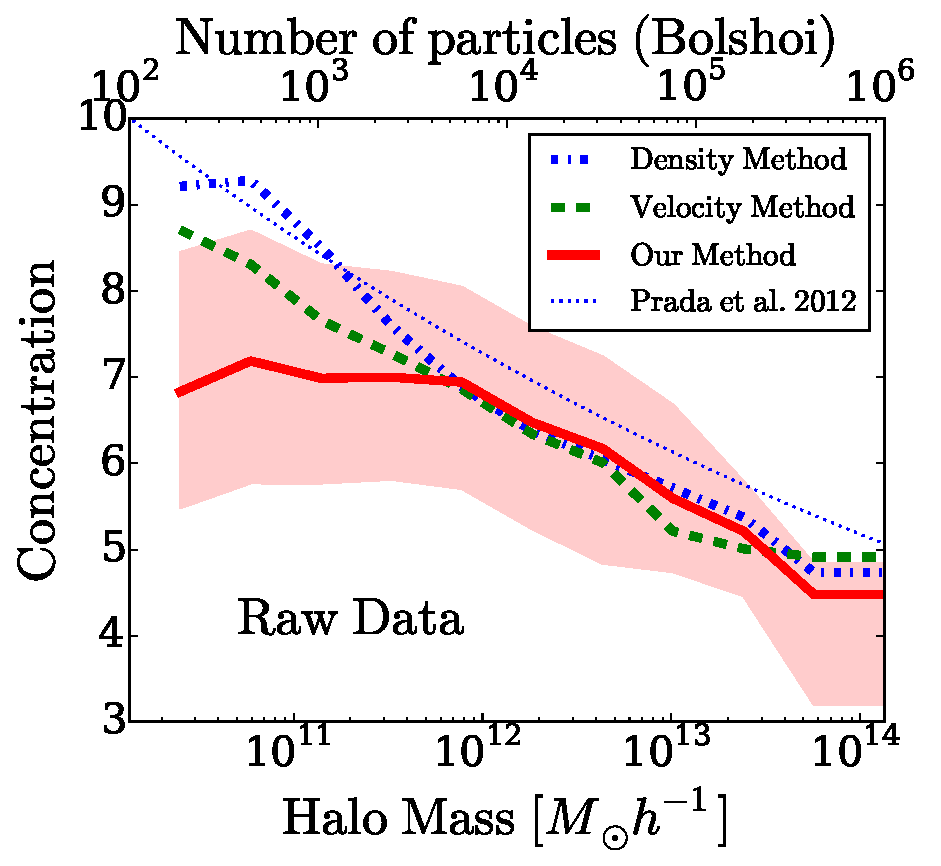
\includegraphics[width=0.45\textwidth]{concentration_bolshoi.pdf}
  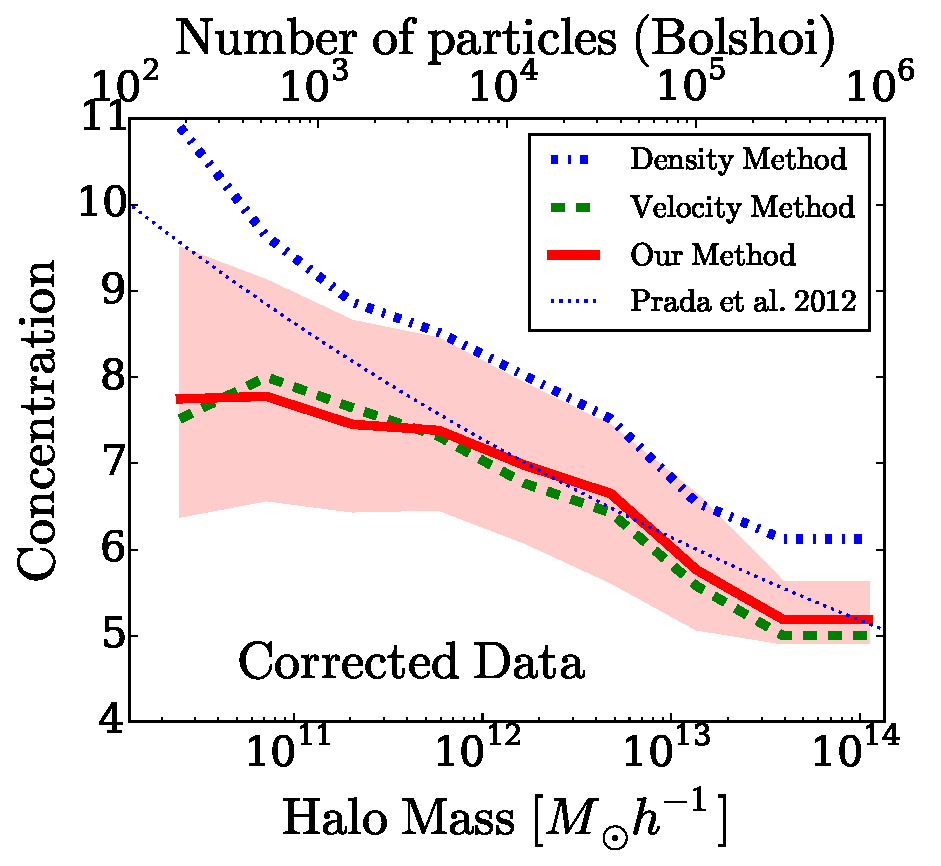
\includegraphics[width=0.45\textwidth]{concentration_bolshoi_corrected.pdf}
\end{center}
\vspace{-0.5cm}
\caption{Mass-concentration relationship for the three different
  methods used on the same cosmological N-body data. 
  All halos are used regardless of their relaxation state.
  The lines correspond to the median concentration values in each mass bin.
  The shaded region presents 10 and 90 per cent spread.
  For clarity we only show the spread for the concentrations estimated
  using the new method. The other two methods have a similar spread. The
  dotted line corresponds to fits reported by \citep{Prada2012}.
  \label{fig:concentration}}
\end{figure*}


The results presented in the previous section show that in an
idealized setup (pure NFW density profiles, perfect spherical halos in
total isolation) the new method performs better than the other two
methods commonly used in the literature.

However, simulated dark matter halos in a cosmological context are
complex. 
They are not isolated, many of them  experience mergers that take them
out of the equilibrium. 
Halos may have also plenty of substructure. 
All these effects disturb the mass density profile, taking it  away
from the ideal NFW profile. 
In order to explore the performance of the new method in this setting, we
use it to estimate the  concentration parameter in dark matter halos
obtained from a cosmological N-body simulation and compare it with the
other two classical methods.   
 
We use data from the MultiDark cosmological simulation that follows
the non-linear evolution of a dark matter density field sampled with
$2048^3$ particles over a cubic box of $1000\ \hMpc$ on a side.  
The data is publicly available at \url{http://www.cosmosim.org/}.
More details about the structure of the database and the simulation
can be found in \citep{2013AN....334..691R}.

We use a halo sample containing all the halos located in a cubic
sub-volume of $100$ \hMpc\ on a side centered on the most massive halo
in the simulation at $z=0$.
This dataset corresponds to the \texttt{miniMDR1}
table in the  database.  
From this sample we select all the halos at $z=0$ detected
with a Friends-of-Friends (FoF) algorithm with masses in the interval
$10^{12}\leq M_{\rm FoF}/\hMsun \leq 10^{14}$.  
The FoF algorithm used a linking length of $0.17$ times the mean
inter-particle distance. This choice translates into an overdensity
$\Delta_h\sim  400-700$ dependent on the halo concentration \citep{More2011}.
Finally, we select from the database all the particles that belong to
each FoF group.

From this set of particles we follow the procedure spelled out in
Section \ref{sec:method} with $\Delta_h=740$ (corresponding to $200$
times the critical density) to select an spherical region that we
redefine to be our halo.  
This choice makes that the overdensities are fully included inside the
original FoF particle group.   
On the interest of providing a fair comparison against the density method we
only report results from overdensities with at least $200$ particles. 

Figure \ref{fig:comparison} shows the comparison between the
concentration values obtained by the three different methods. 
The diagonal line marks a one-to-one correspondence if all the values
were equal.
The three methods show a broad general agreement. 
The largest difference is present at high concentration $c>5$ where
the new method produces systematic lower values than the other two
methods. Most of the differences are at the $20\%$ level, with some
extreme cases for the highest concentration values with $50\%$
differences.  The velocity and density methods produce consistent
values within a $20\%$ scatter, only some halos with very high
concentrations $c\sim 10$ have a $15\%$ lower concentration with the
velocity method. 

We explored halo shape and relaxation as a source of this
differences. We found that shape does not bias the concentration
estimation; relaxation, quantified by the
offset between the center of mass and minimum of the potential, can
only offset at most $5\%$ the median results between methods.  
We note that the highest concentration values correspond to the smallest halos
with $\sim 200$ particles, a regime where both the density and
velocity methods are reliable only the $5\%$ in a perfect spherical
halo.  

The differences we find might signal a deviation from the NFW profile
due to the low resolution of these halos. We suggest that asserting
with confidence the systematic difference between the different
methods should be confirmed  a higher resolution simulation and larger
statistics. We leave this comparison for future work.  
  

Figure \ref{fig:concentration} summarizes the previous results in the
mass-concentration relationship. 
We find that the median concentration
can be fit by the following relationship
\begin{equation} c_{200} = 5.62 \left(\frac{M_{200}}{10^{12}\hMsun}\right)^{-0.061}, 
\end{equation}
%
which has a similar power value compared to the $-0.075$ reported by
\citep{Prada2012}, while the normalization is $\sim 20\%$ lower
compared to the $7.28$ value reported by the same authors. 



\section{Conclusions}
\label{sec:conclusions}

In this letter we presented a new method to estimate the concentration
of dark matter halos in N-body simulations.  
We tested the method on mock halo data to study the impact of total
number of particles and input concentration on the retrieved values.  
We compared these results against two other methods commonly used in
the literature to estimate concentrations.  
For all methods, the accuracy in retrieving the input concentration
increases with the number of particles as summarized in Figure
\ref{fig:error}.  The new method systematically outperforms the other two.

We also applied the method to halos extracted from a cosmological
N-body simulation to estimate the impact on the mass concentration
relationship. Although the three  methods are in broad agreement there
are some noticeable differences in the mass concentration relationship
at lower masses, $<10^{13}\hMsun$, at the $20-30\%$ level.

These are encouraging results. They show that using the integrated
mass profile to find the DM halo concentration is a tool deserving
deeper scrutiny. Further tests with larger simulated volumes, varying
numerical resolution and different density profiles are
the next natural step to explore the full potential of this
new method. 

\vspace{0.5cm}

 The authors acknowledge the technical support from the new
 high-performance computing facility at Uniandes. JEF-R acknowledges
 financial support from Vicerrector\'ia de Investigaciones at Uniandes
 through a FAPA project. JCMC acknowledges financial support from
 ``Estrategia de  sostenibilidad 2014-2015, Universidad de
 Antioquia''.    

\bibliographystyle{mn2e}
%\bibliography{references}
\begin{thebibliography}{}

\bibitem[\protect\citeauthoryear{{Duffy}, {Schaye}, {Kay} \& {Dalla
  Vecchia}}{{Duffy} et~al.}{2008}]{Duffy2008}
{Duffy} A.~R.,  {Schaye} J.,  {Kay} S.~T.,    {Dalla Vecchia} C.,  2008,
  \mnras, 390, L64

\bibitem[\protect\citeauthoryear{{Foreman-Mackey}, {Hogg}, {Lang} \&
  {Goodman}}{{Foreman-Mackey} et~al.}{2013}]{emcee}
{Foreman-Mackey} D.,  {Hogg} D.~W.,  {Lang} D.,    {Goodman} J.,  2013, \pasp,
  125, 306

\bibitem[\protect\citeauthoryear{{Klypin}, {Yepes}, {Gottlober}, {Prada} \&
  {Hess}}{{Klypin} et~al.}{2014}]{Klypin2014}
{Klypin} A.,  {Yepes} G.,  {Gottlober} S.,  {Prada} F.,    {Hess} S.,  2014,
  ArXiv e-prints

\bibitem[\protect\citeauthoryear{{Ludlow}, {Navarro}, {Angulo},
  {Boylan-Kolchin}, {Springel}, {Frenk} \& {White}}{{Ludlow}
  et~al.}{2014}]{Ludlow2014}
{Ludlow} A.~D.,  {Navarro} J.~F.,  {Angulo} R.~E.,  {Boylan-Kolchin} M.,
  {Springel} V.,  {Frenk} C.,    {White} S.~D.~M.,  2014, \mnras, 441, 378

\bibitem[\protect\citeauthoryear{{Macci{\`o}}, {Dutton} \& {van den
  Bosch}}{{Macci{\`o}} et~al.}{2008}]{Maccio2008}
{Macci{\`o}} A.~V.,  {Dutton} A.~A.,    {van den Bosch} F.~C.,  2008, \mnras,
  391, 1940

\bibitem[\protect\citeauthoryear{{More}, {Kravtsov}, {Dalal} \&
  {Gottl{\"o}ber}}{{More} et~al.}{2011}]{More2011}
{More} S.,  {Kravtsov} A.~V.,  {Dalal} N.,    {Gottl{\"o}ber} S.,  2011, \apjs,
  195, 4

\bibitem[\protect\citeauthoryear{{Mu{\~n}oz-Cuartas}, {Macci{\`o}},
  {Gottl{\"o}ber} \& {Dutton}}{{Mu{\~n}oz-Cuartas} et~al.}{2011}]{Munoz2011}
{Mu{\~n}oz-Cuartas} J.~C.,  {Macci{\`o}} A.~V.,  {Gottl{\"o}ber} S.,
  {Dutton} A.~A.,  2011, \mnras, 411, 584

\bibitem[\protect\citeauthoryear{{Navarro}, {Frenk} \& {White}}{{Navarro}
  et~al.}{1997}]{NFW}
{Navarro} J.~F.,  {Frenk} C.~S.,    {White} S.~D.~M.,  1997, \apj, 490, 493

\bibitem[\protect\citeauthoryear{{Navarro}, {Ludlow}, {Springel}, {Wang},
  {Vogelsberger}, {White}, {Jenkins}, {Frenk} \& {Helmi}}{{Navarro}
  et~al.}{2010}]{Navarro2010}
{Navarro} J.~F.,  {Ludlow} A.,  {Springel} V.,  {Wang} J.,  {Vogelsberger} M.,
  {White} S.~D.~M.,  {Jenkins} A.,  {Frenk} C.~S.,    {Helmi} A.,  2010,
  \mnras, 402, 21

\bibitem[\protect\citeauthoryear{{Neto}, {Gao}, {Bett}, {Cole}, {Navarro},
  {Frenk}, {White}, {Springel} \& {Jenkins}}{{Neto} et~al.}{2007}]{Neto2007}
{Neto} A.~F.,  {Gao} L.,  {Bett} P.,  {Cole} S.,  {Navarro} J.~F.,  {Frenk}
  C.~S.,  {White} S.~D.~M.,  {Springel} V.,    {Jenkins} A.,  2007, \mnras,
  381, 1450

\bibitem[\protect\citeauthoryear{{Prada}, {Klypin}, {Cuesta}, {Betancort-Rijo}
  \& {Primack}}{{Prada} et~al.}{2012}]{Prada2012}
{Prada} F.,  {Klypin} A.~A.,  {Cuesta} A.~J.,  {Betancort-Rijo} J.~E.,
  {Primack} J.,  2012, \mnras, 423, 3018

\bibitem[\protect\citeauthoryear{{Riebe}, {Partl}, {Enke}, {Forero-Romero},
  {Gottl{\"o}ber}, {Klypin}, {Lemson}, {Prada}, {Primack}, {Steinmetz} \&
  {Turchaninov}}{{Riebe} et~al.}{2013}]{2013AN....334..691R}
{Riebe} K.,  {Partl} A.~M.,  {Enke} H.,  {Forero-Romero} J.,  {Gottl{\"o}ber}
  S.,  {Klypin} A.,  {Lemson} G.,  {Prada} F.,  {Primack} J.~R.,  {Steinmetz}
  M.,    {Turchaninov} V.,  2013, Astronomische Nachrichten, 334, 691

\end{thebibliography}

\end{document}


